%% CAPITULO 4
\hypertarget{estilo:capitulo}{}
\chapter{ESTUDO DE CASO DE COMPLEXO CONVECTIVO DE MESOESCALA}
\label{ss:cap4}

Durante o período do projeto SALLJEX, foram identificados em torno de 100 SCMs entre as bacias Amazônica e do Prata, no Altiplano Sul-americano. No mês de Janeiro de 2003, ocorreram dois casos de CCMs, o primeiro no dia 18 de Janeiro e o segundo no dia 23 de Janeiro. Autores como \citeonline{zipseretal04} estudaram estes eventos e outros estudos numéricos foram realizados com o objetivo de se verificar se os modelos de PNT eram capazes de simular as principais características dos CCMs. \citeonline{paegleetal04} comparam vários modelos regionais, dentre eles versões diferentes dos modelos RAMS, MM5 e Eta (incluindo o modelo regional operacional, na época, do CPTEC - Eta 40 km). Os autores mostram que existe uma grande variação entre as previsões dos diferentes modelos e apontam as possíveis causas como sendo condições iniciais e de contorno não muito realistas, dados de baixa qualidade, dinâmica e parametrizações físicas inadequadas para a simulação desse tipo de fenômenos meteorológicos em regiões específicas do globo. Neste mesmo caso, os autores mostram também, como exemplo, o caso do CCM ocorrido no dia 18 de Janeiro em que os modelos regionais não foram capazes de simular as principais características do CCM. Em altas resoluções (e.g., 20 km), os modelos regionais são capazes de prever grandes acumulados de precipitação, mas, no entanto, não refletem bem as características associada aos SCMs. \citeonline{paegleetal04} ainda apontam para o fato de que a inicialização e a validação dos modelos pode beneficiar a análises geradas pelos modelos de previsão.

Para este estudo de caso, foi escolhido o CCM ocorrido no dia 23 de janeiro de 2003. Em \citeonline{rozantecavalcanti06} são feitas simulações sobre o CCM do dia 18 de Janeiro de 2003 e outros experimentos numéricos com o modelo Eta durante o período da campanha do SALLJEX. Além disso, como parte do estudo de caso, busco-se verificar se o sistema Eta+RPSAS foi hábil na detecção de um caso de Jato de Baixos Níveis ocorrido entre os dias 20 e 21 de Janeiro de 2003, antes do caso de CCM. Esse caso de JBN também já foi estudado por \citeonline{soaresmarengo04}.

A \autoref{fig59} mostra a série temporal da seção vertical do vento meridional da Reanálise 2 do NCEP/DOE e dos experimentos SAP e CAP para o nível de 850 hPa para a cidade de Santa Cruz (Bolívia), na latitude próxima a 17,6ºS e longitude próxima a 63ºW.

\begin{figure}
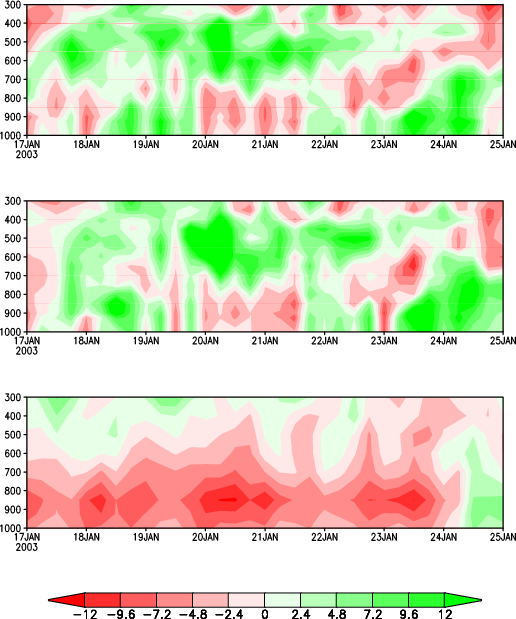
\includegraphics[height=14cm]{./figs/jatos.png}
\centering
\caption{Série temporal da seção vertical da componente meridional do vento em 850 hPa para os experimentos SAP (primeira linha), CAP (segunda linha) e reanálise do NCEP (terceira linha), próxima a Santa Cruz na Bolívia (17,6ºS e 63ºW).}
\label{fig59}
\end{figure}

A identificação do JBN foi feita com a aplicação dos critérios de Bonner \cite{bonner68} adaptados para a AS. Estes critérios levam em consideração que a magnitude do vento em torno de 850 hPa deve ser superior a 12 ms-1, que o cisalhamento do vento entre 850 e 700 hPa deve ser de pelo menos 6 ms-1 e que a componente meridional do vento tem que ser negativa (de norte) e que seu módulo deve ser maior do que o módulo da componente zonal.

Em relação à magnitude do vento, como pode ser visto na \autoref{fig59}, a reanálise do NCEP apresenta ventos superiores a 12 ms-1 entre os dias 20 e 21 de Janeiro. Neste mesmo período, os experimentos mostram um fluxo de vento de menor intensidade e definição. Neste caso, o experimento SAP apresenta valores mais compatíveis com a reanálise do NCEP, se comparado com o experimento CAP.

Na \autoref{fig61} são mostradas as imagens do canal 4 (infravermelho) do satélite GOES 8 (\textit{Geostationary Satellite Server}). Nestas imagens, pode-se observar um CCM que começou a se formar no dia 22 de janeiro de 2003 às 18Z, tendo seu ciclo de vida com duração total de um dia, culminando ao dia 23 de janeiro de 2003 às 12Z. Na \autoref{fig62}, é mostrada a precipitação diária observada do SALLJEX, acumulada às 12Z. Na \autoref{fig63}, a precipitação estimada pelo TRMM para a mesma região.

\begin{figure}
\centering
a)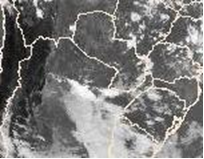
\includegraphics[height=4.3cm]{./figs/sat01.png}\hspace{0.2cm}b)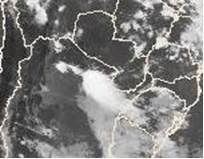
\includegraphics[height=4.3cm]{./figs/sat02.png}\hspace{0.2cm}
c)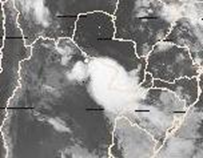
\includegraphics[height=4.3cm]{./figs/sat03.png}\hspace{0.2cm}d)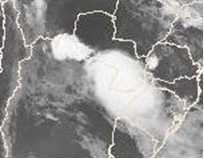
\includegraphics[height=4.3cm]{./figs/sat04.png}
\\[0.15cm]
e)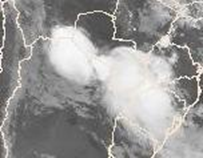
\includegraphics[height=4.3cm]{./figs/sat05.png}\hspace{0.2cm}f)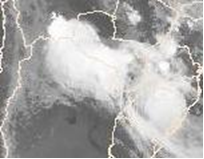
\includegraphics[height=4.3cm]{./figs/sat06.png}\hspace{0.2cm}
g)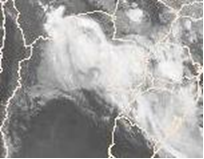
\includegraphics[height=4.3cm]{./figs/sat07.png}\hspace{0.2cm}h)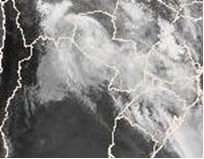
\includegraphics[height=4.3cm]{./figs/sat08.png}
\caption{Imagens do Satélite GOES 8 no canal 4 (infravermelho). Evolução de um complexo convectivo de mesoescala. Nas figuras: a) 20030122$\_$18Z; b) 20030122$\_$21Z; c) 20030123$\_$00Z; d) 20030123$\_$03Z; e) 20030123$\_$06Z; f) 20030123$\_$09Z; g) 20030123$\_$12Z; h) 20030123$\_$15Z.}
\label{fig61}
\end{figure}

\begin{figure}
\centering
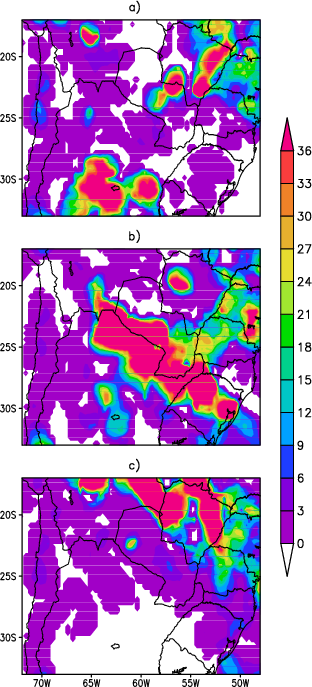
\includegraphics[height=15cm]{./figs/prec_salljex1.png}
\caption{Precipitação observada diária SALLJEX, acumulado 12Z. Nas figuras: a) 20030122$\_$12Z; b) 20030123$\_$12Z; c) 20030124$\_$12Z.}
\label{fig62}
\end{figure}


Com as simulações dos experimentos SAP e CAP, buscou-se observar se o modelo de previsão Eta e o sistema de assimilação de dados RPSAS foram capazes de simular esse complexo convectivo, através da simulação dos seguintes parâmetros: ciclo de vida (duração), intensidade, posicionamento e precipitação associada.

Diante das configurações ajustadas para o modelo de previsão Eta (com e sem a assimilação de precipitação, com filtro digital e no modo hidrostático), e comparando-se o resultado dos experimentos com os dados do SALLJEX e do TRMM, pode-se notar que sem a assimilação de precipitação (experimento SAP), o modelo não foi capaz de reproduzir o evento de precipitação ocasionado pelo CCM. Apenas com a assimilação de precipitação (experimento CAP), o modelo foi capaz de reproduzir a precipitação ocasionada pelo CCM.

Para efeito de comparação, vale lembrar que durante o experimento de campo do SALLJEX, foram instalados vários pluviógrafos adicionais na região de estudo o que favoreceu uma descrição muito mais minuciosa dos acumulados de precipitação. A precipitação do TRMM3B42, embora possua uma resolução temporal mais refinada (3 horas), mostra que em seus acumulados uma distribuição de precipitação mais discreta do que a do SALLJEX, principalmente às 06Z do dia 23 de Janeiro de 2003, quando o CCM atinge seu estágio maduro. O campo de precipitação produzido pelo modelo Eta, com o experimento CAP, apresenta também taxas de precipitação inferiores àquelas observadas no SALLJEX, embora sua distribuição espacial seja concordante com o que foi encontrado na observação.

Observando-se as imagens do canal infravermelho do GOES 8, nota-se que o CCM começou a se formar às 18Z do dia 22 de Janeiro e atinge o seu estágio maduro (o máximo de precipitação) às 06Z do dia 23, quando observa-se os critérios de forma tamanho e tempo de duração definidos por \citeauthoronline{maddox80} para a caracterização do CCM.

As imagens da \autoref{fig63} mostram a precipitação estimada do TRMM correspondentes às imagens de satélite do GOES 8.

\begin{figure}[!hpb]
\centering
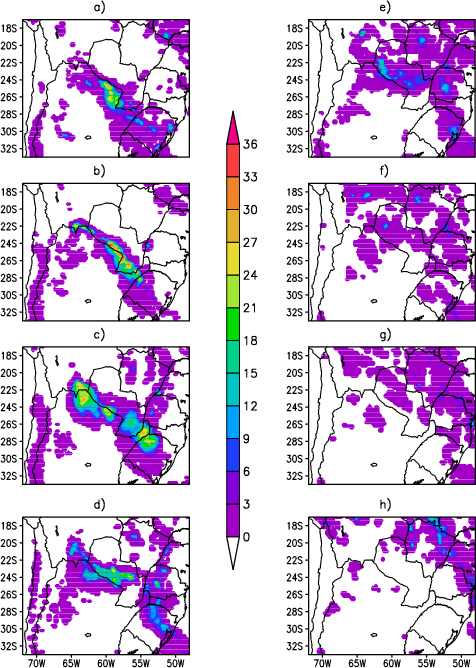
\includegraphics[height=15cm]{./figs/prec_trmm3b42.png}
\caption{Precipitação Estimada (TRMM3B42). Evolução de um complexo convectivo de mesoescala. Nas figuras: a) 20030123$\_$00Z; b) 20030123$\_$03Z; c) 20030123$\_$06Z; d) 20030123$\_$09Z; e) 20030123$\_$12Z; f) 20030123$\_$15Z; g) 20030123$\_$18Z; h) 20030123$\_$21Z.}
\label{fig63}
\end{figure}

Nota-se que 6 horas após (09Z do dia 23) o máximo de precipitação do CCM (06Z do dia 23), embora o CCM ainda apresente suas características principais, a precipitação do TRMM apresenta taxas relativamente menores do que o observado pelo SALLJEX no acumulado das 12Z do dia 23. 

Os campos de precipitação produzidos pelo modelo Eta com os experimentos SAP e CAP, mostram diferenças significativas durante as previsões de 6, 12, 18 e 24 horas. A assimilação dos dados de precipitação fez com que o modelo Eta reproduzisse de forma relativamente satisfatória o campo de precipitação apresentado na imagem ``c'' da \autoref{fig64}. No entanto, levando-se em consideração os esquemas físicos do modelo,  a melhor discretização dos tipos de solo do modelo de superfície NOAH e o esquema de convecção BMJ, nota-se também que as simulações do experimento CAP tendem a superestimar e a espalhar um pouco mais a precipitação nos horários subsequentes à 06Z do dia 23 de Janeiro.

\begin{figure}[!hpb]
\centering
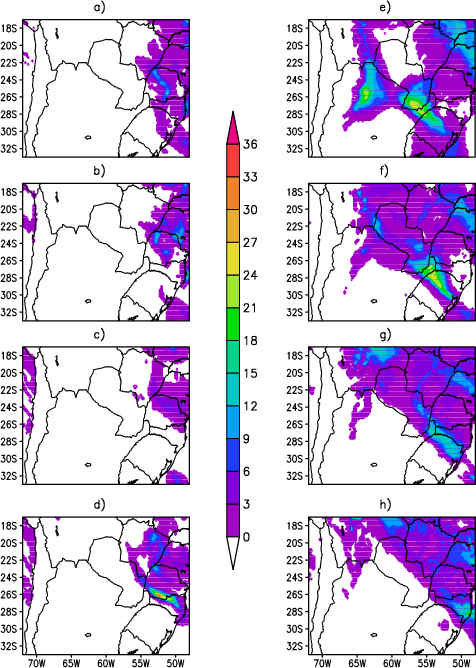
\includegraphics[height=15cm]{./figs/prec_eta1.png}
\caption{Precipitação Prevista pelo sistema Eta+RPSAS a partir do dia 23/01/2003. Nas figuras: (primeira coluna) previsões de a) 6h; b) 12h; c) 18h e d) 24h para o experimento SAP, (segunda coluna) previsões e) 6h; f) 12h; g) 18h e h) 24h para o experimento CAP.}
\label{fig64}
\end{figure}

A próxima \autoref{fig65} mostra os perfis verticais do vento meridional entre os níveis de 1000 hPa e 250 hPa. Nesta figura são mostrados os perfis de vento para os dois experimentos testados (SAP e CAP) e o perfil de vento da Reanálise 2 do NCEP/DOE para a latitude de 22ºS (próximo à localidade de Mariscal no Paraguai - não mostrado) onde ocorreu o CCM. 

\begin{figure}[!hpb]
\centering
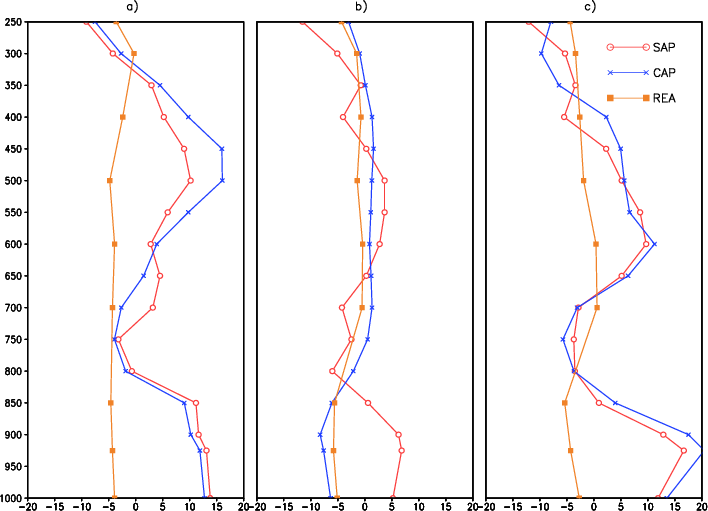
\includegraphics[height=10.5cm]{./figs/perf_vert_vento.png}
\caption{Perfis do vento meridional na latitude de 22ºS, próximo à localidade de Mariscal. Em amarelo a Reanálise 2 do NCEP/DOE, em azul o experimento CAP e em vermelho o experimento SAP. Na imagem da esquerda: 18Z do dia 22 de Janeiro. Na imagem do centro: 00Z do dia 23 de Janeiro e na imagem da direita, as 06Z do dia 23 de Janeiro. Unidades estão em m/s.}
\label{fig65}
\end{figure}

Os perfis de vento meridional mostram nos horários anteriores à ocorrência do CCM, os dois experimentos (SAP e CAP) mostravam-se concordantes quanto à intensidade, superestimando a intensidade apresentada pelo vento da reanálise. Já no horário referente ao estágio de maturação do CCM (às 06Z do dia 23), observa-se que o experimento SAP coloca o vento no sentido contrário do que é apresentado pela reanálise e pelo experimento CAP. \citeonline{herdiesetal07} apresenta os mesmos perfis de vento meridional para a latitude de 22ºS juntamente com as observações de vento do SALLJEX. Os resultados apresentados pelo experimento CAP concordam em direção e intensidade (do vento) com o que foi simulado pelos modelos globais do NCEP.

A \autoref{fig66} mostra a seção vertical do fluxo de umidade também para a latitude de 22ºS. Nesta figura são mostrados os resultados encontrados para os experimentos SAP (primeira linha) e CAP (segunda linha). Nesta figura nota-se que o fluxo de umidade apresentado pelo experimento CAP às 06Z do dia 23 apresenta valores elevados (da ordem de 100 g/kg m/s).

\begin{figure}
\centering
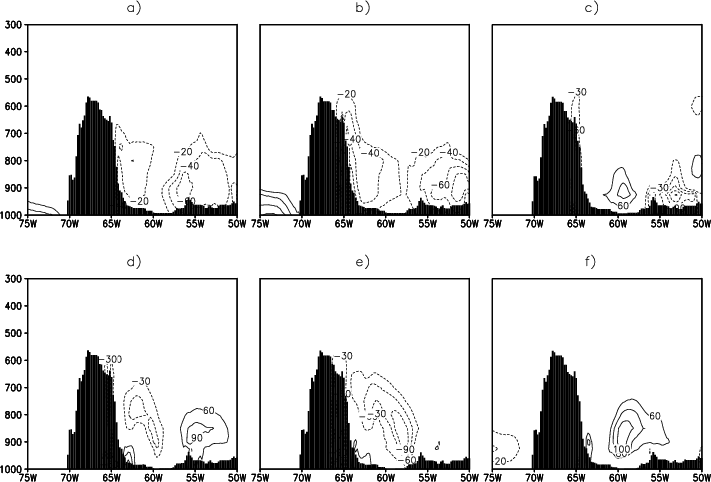
\includegraphics[height=10.5cm]{./figs/sec_vert_flux_umi.png}
\caption{Seção vertical do fluxo de umidade ($qv$) ao longo da latitude de 22ºS, às 18Z do dia 22 (coluna da esquerda - letras ``a'' e ``d''), às 00Z do dia 23 (coluna do meio - ``b'' e ``e'') e às 06Z do dia 23 de Janeiro (coluna da direita - letras ``c'' e ``f''). Os contornos estão em g/kg m/s.}
\label{fig66}
\end{figure}

A \autoref{fig67} mostra os campos de velocidade vertical (Omega) em 700 hPa para os experimen-tos SAP e CAP e a precipitação do SALLJEX. Comparando-se os dois experimentos, nota-se que o experimento CAP foi capaz de detalhar melhor o desenvolvimento vertical das nuvens convectivas associadas ao CCM. Os contornos em azul-claro representam valores de -0.2 Pa/s. Em \citeonline{herdiesetal07} estes valores são de -0.5 Pa/s.
 
\begin{figure}
\centering
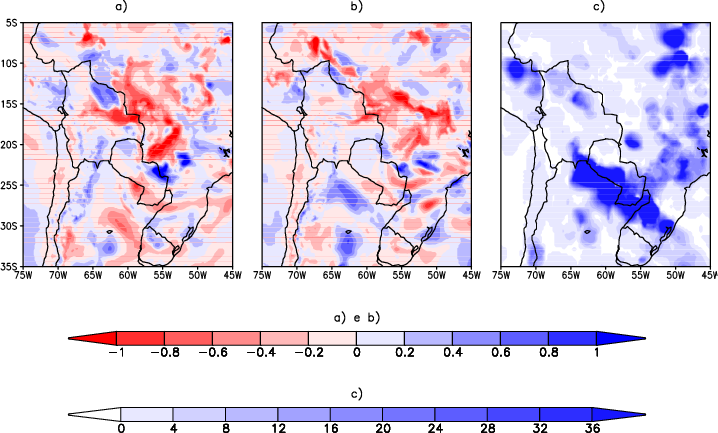
\includegraphics[height=8.5cm]{./figs/vel_vert_omega_salljex.png}
\caption{Velocidade vertical em 700 hPa para os experimentos a) SAP e b) CAP. Em ambos os casos são mostradas as previsões de 6 horas. Em c) precipitação observada do SALLJEX. Os contornos em azul-claro apresentam valores iguais a -0.2 Pa/s.}
\label{fig67}
\end{figure}
